% Seminar deck. Compile: cd slides && latexmk   (settings in .latexmkrc, output in build/)
% Detailed version with results up front: main_results.tex.
% tab02_total.tex is written by code/build/slides_tables.py; figures from output/omxsb_replication_2007/.
\documentclass[aspectratio=169]{beamer}
\usetheme{default}
\setbeamercolor{structure}{fg=red!75!black}
\setbeamertemplate{navigation symbols}{}
\setbeamertemplate{itemize items}[triangle]
\setbeamerfont{subtitle}{shape=\itshape,size=\large}
\setbeamercolor{author in head/foot}{fg=black}
\setbeamercolor{title in head/foot}{fg=white,bg=red!75!black}
\setbeamercolor{date in head/foot}{fg=black}
\setbeamerfont{author in head/foot}{size=\scriptsize}
\setbeamerfont{title in head/foot}{size=\scriptsize}
\setbeamerfont{date in head/foot}{size=\scriptsize}
\setbeamertemplate{footline}{%
  \leavevmode\hbox{%
  \begin{beamercolorbox}[wd=.3333\paperwidth,ht=2.25ex,dp=1ex,center]{author in head/foot}%
    \usebeamerfont{author in head/foot}\insertshortauthor
  \end{beamercolorbox}%
  \begin{beamercolorbox}[wd=.3333\paperwidth,ht=2.25ex,dp=1ex,center]{title in head/foot}%
    \usebeamerfont{title in head/foot}\insertshorttitle
  \end{beamercolorbox}%
  \begin{beamercolorbox}[wd=.3334\paperwidth,ht=2.25ex,dp=1ex,right]{date in head/foot}%
    \usebeamerfont{date in head/foot}\insertshortdate\hspace*{4em}%
    \insertframenumber\,/\,\inserttotalframenumber\hspace*{2ex}
  \end{beamercolorbox}}%
  \vskip0pt}
\usepackage{appendixnumberbeamer}
\usepackage{booktabs}
\usepackage{graphicx}
\usepackage{amsmath}
\usepackage{hyperref}
\graphicspath{{../output/omxsb_replication_2007/figures/}}
\newcommand{\src}[1]{{\scriptsize\color{gray}#1\par}}

\title[Finance Thesis Fall 26]{Pre-announced, uninformed, and large}
\subtitle{Has the index effect disappeared in Sweden?}
\author[Alexander Fox \& Ludvig P Uväng]{Alexander Fox \and Ludvig Pauli Uväng}
\institute{Stockholm School of Economics}
\date{December 2026}

\begin{document}

\maketitle

% ---------------------------------------------------------------- Question
\begin{frame}{Research question}
  Has the index effect disappeared in Sweden as it has in the US, and why?

  \bigskip
  Subquestions:
  \begin{enumerate}
    \item Has the OMXSB index effect changed from 2007 to 2026, and which of
      Greenwood and Sammon's five explanations fit?
    \item When the state moves pension money out of a fund, the decision comes
      months before the sale. Does the price move at the decision or at the sale?
  \end{enumerate}
\end{frame}

% ---------------------------------------------------------------- Background
\begin{frame}{Background: 2000--2018}
  \begin{itemize}
    \item \textbf{2000:} 2.5\% of wages go to the premium pension system,
      invested in picks from the platform; if not chosen $\rightarrow$ AP7
    \item \textbf{2000--2018:} initial choices were untouched more than a decade
      later (Cronqvist, Thaler and Yu 2018); letters from the PPM about bad and
      expensive funds were ignored (Kinnerud and Lorentzon 2026)
  \end{itemize}
\end{frame}

\begin{frame}{Background: the open platform, 2016--2018}
  \begin{itemize}
    \item The open platform let many funds in. By 2016 there were 850 funds,
      two of which were Falcon and Allra
    \item Falcon (2 BSEK) put it into assets connected to its own owners
    \item Allra charged savers for worthless derivative trades through a Dubai subsidiary
    \item Both had marketed aggressively by phone to savers who did not understand
      what they were buying
  \end{itemize}
\end{frame}

\begin{frame}{Background: new law and the 2019 purge}
  \begin{itemize}
    \item \textbf{2018:} new law: three-year track record, at least 500 MSEK AUM,
      no phone sales, a signed agreement with PPM under new terms
    \item \textbf{2019:} a purge that removed 313 funds, 84 BSEK moved, 97\% by default
    \item Platform was still open
  \end{itemize}
\end{frame}

\begin{frame}{Background: Fondtorgsnämnden and the procurements}
  \begin{itemize}
    \item \textbf{2019--2022:} Fondtorgsnämnden is created and procures the funds;
      PPM handles all administration
    \item \textbf{2024--2026:} eleven awards: Europe, Global Index, Nordic Active,
      Swedish Active, Swedish Index, Global Active (pending due to the Indecap
      appeal), Swedish Small Cap
    \item A fund that loses is emptied on set days; the award is public months
      before
  \end{itemize}
\end{frame}

% ---------------------------------------------------------------- Anchor
\begin{frame}{Anchor: Greenwood and Sammon (2025, JF)}
  \begin{itemize}
    \item When a stock joins the S\&P 500, index funds must buy it on a known day
    \item Additions rose 7.4\% from announcement to effective date in the 1990s,
      0.3\% in the 2010s, not distinguishable from zero
    \item Deletions fell 16\% in the 1990s and 0.1\% in the 2010s
    \item Why did it disappear? They test five explanations
  \end{itemize}
\end{frame}

\begin{frame}{Anchor: five explanations}
  \begin{enumerate}
    \item \textbf{Composition:} added firms are smaller relative to the index, more
      liquid. Explains a little
    \item \textbf{Migrations:} additions come from the MidCap, whose trackers sell
      as S\&P 500 trackers buy. Explains part
    \item \textbf{Predictability:} traders buy months ahead. Long pre-announcement
      returns rose, the 20-day window did not. Small role
    \item \textbf{General liquidity:} spreads fell. Some role
    \item \textbf{Event liquidity:} other institutions supply the stock on the day.
      The main story
  \end{enumerate}
  \bigskip
  \textbf{Their verdict:} migrations plus the market's learned ability to supply liquidity
\end{frame}

% ---------------------------------------------------------------- Replication
\begin{frame}{Replication on OMXSB, 2007--2026}
  \begin{itemize}
    \item Every addition and deletion, 39 reviews, 536 events
    \item The same windows and the same market-adjusted return
    \item Five subperiods instead of four decades; then their five tests
  \end{itemize}
  \begin{align}
    AR_{it} &= R_{it} - R_{m,t} \\
    \text{Total Return}_i &= \sum_{t=AD_i-1}^{ED_i+1} AR_{it}
  \end{align}
  \src{(1) G\&S eq. 3, $R_m$ = the OMXSB index. (2) G\&S pp. 9--10, the day before the
  announcement to the day after the change; summing is our choice.}
\end{frame}

\begin{frame}{Replication: demand and price}
  \begin{align}
    \text{Net Trading}_{i,t} &= 100 \times \frac{\text{Shares held}_{i,t+1} - \text{Shares held}_{i,t-1}}{\text{Shares outstanding}_{i,t+1}} \\
    \text{Total Return}_i &= a + b\,\text{Net Trading}_i + e_i
  \end{align}
  \src{(3) G\&S eq. 2; shares held by index funds, from FI's quarterly holdings 2019--2026.
  (4) G\&S Fig. 3; reporting $b$ with a standard error is our addition.}
\end{frame}

% ---------------------------------------------------------------- Extension
\begin{frame}{Extension: the same test on the FTN sales}
  \begin{itemize}
    \item When a fund loses a procurement, the state redeems the savers' units on
      days set in advance and the fund sells its stocks. Forced, uninformed and
      pre-announced, like an index deletion
    \item The award is months before the sale, so a move at the award is
      predictability and a move at the sale is event liquidity
  \end{itemize}
  \begin{align}
    \text{Net Trading}_{i,r} &= -100 \times \frac{\sum_{f \in L_r} \rho_{f,r}\, TNA_{f,r}\, w_{f,i}}{MCAP_{i,r}} \\
    CAR^{j}_{i,r} &= a^{j} + b^{j}\,\text{Net Trading}_{i,r} + e_{i,r}, \qquad j \in \{A, E\}
  \end{align}
  \src{(5) ours, in the unit of (3): $L_r$ = losing funds in round $r$, $\rho$ = share redeemed,
  $TNA$ = fund assets, $w$ = the stock's weight in the fund. (6) ours, the form of (4):
  $A$ = award window, $E$ = sale window. $b^A$ and $b^E$ are compared with $b$ from (4) for deletions.}
\end{frame}

% ---------------------------------------------------------------- Data
\begin{frame}{Data}
  \centering\small
  \begin{tabular}{ll}
    \toprule
    Source & Coverage \\
    \midrule
    Nasdaq OMXSB changes & 39 reviews, 2007 to 2026 \\
    LSEG daily stock panel & 2,117 series, 2005 to 2026 \\
    FI quarterly holdings & 31 quarters, 2018 to 2026 \\
    FTN procurement reports & 11 rounds \\
    Pensionsmyndigheten monthly fund files & 53\,000 fund months, 2018--2026 \\
    Morningstar daily fund data & 78 losers \\
    Pensionsmyndigheten order log & requested \\
    \bottomrule
  \end{tabular}
\end{frame}

% ---------------------------------------------------------------- Status
\begin{frame}{Where we are}
  \begin{itemize}
    \item \textbf{Replication done:} Table 2 on 487 events over 39 reviews,
      2007 to 2026, with the five tests (appendix)
    \item \textbf{First result:} the effect was there in 2007--2012 and is weaker
      since; no period after 2017 can be told from zero
    \item \textbf{Event data built:} every OMXSB change with announcement and
      effective dates; prices, FI holdings and fund files collected
    \item \textbf{FTN mapped:} every round, award date and losing fund
    \item \textbf{Order log} requested from Pensionsmyndigheten
  \end{itemize}
\end{frame}

\begin{frame}{What is left}
  \begin{itemize}
    \item \textbf{Design file:} equations (5) and (6), the windows and the clustering,
      committed and signed off before any FTN return is computed
    \item \textbf{Extension:} build the dose per stock and round, run (6) once
    \item \textbf{Writing} runs alongside: background and literature in progress
  \end{itemize}
\end{frame}

\appendix
\setbeamertemplate{footline}{}
\begin{frame}[plain]
  \centering\LARGE APPENDIX
\end{frame}

\begin{frame}{Hypotheses for the extension}
  \begin{itemize}
    \item $H_A$: $b^A \approx b$, $b^E \approx 0$. The price moves when the sale
      becomes predictable
    \item $H_E$: $b^A \approx 0$, $b^E \approx b$. The price moves when the stock
      is sold; a flow nobody has learned to supply is not absorbed
    \item $H_0$: $b^A \approx b^E \approx 0$. The market absorbs the flow
  \end{itemize}
\end{frame}

\begin{frame}{Table 2: total return by period}
  \centering\small
  \begin{tabular}{lrrrrr}
\toprule
 & 2007–2012 & 2013–2017 & 2018–2020 & 2021–2023 & 2024–2026 \\
\midrule
\textbf{Additions} & 5.80*** & 2.21 & 2.43 & 0.51 & 2.67 \\
 & (1.35) & (1.43) & (1.59) & (1.01) & (1.88) \\
 & \{0.04\} & \{0.28\} & \{0.04\} & \{0.52\} & \{0.03\} \\
$N$ & 45 & 57 & 50 & 59 & 45 \\
\addlinespace
\textbf{Deletions} & -3.01** & -5.49*** & 0.88 & -1.45* & -2.69*** \\
 & (1.35) & (1.79) & (1.54) & (0.81) & (0.90) \\
 & \{0.36\} & \{0.01\} & \{0.66\} & \{0.41\} & \{0.16\} \\
$N$ & 58 & 36 & 38 & 54 & 39 \\
\bottomrule
\end{tabular}


  \medskip\raggedright\footnotesize
  Mean CAR in percent, HC1 standard error in parentheses, wild cluster bootstrap p-value in braces.
\end{frame}

\begin{frame}{Run-up before the announcement (anchor Figure 8)}
  \begin{center}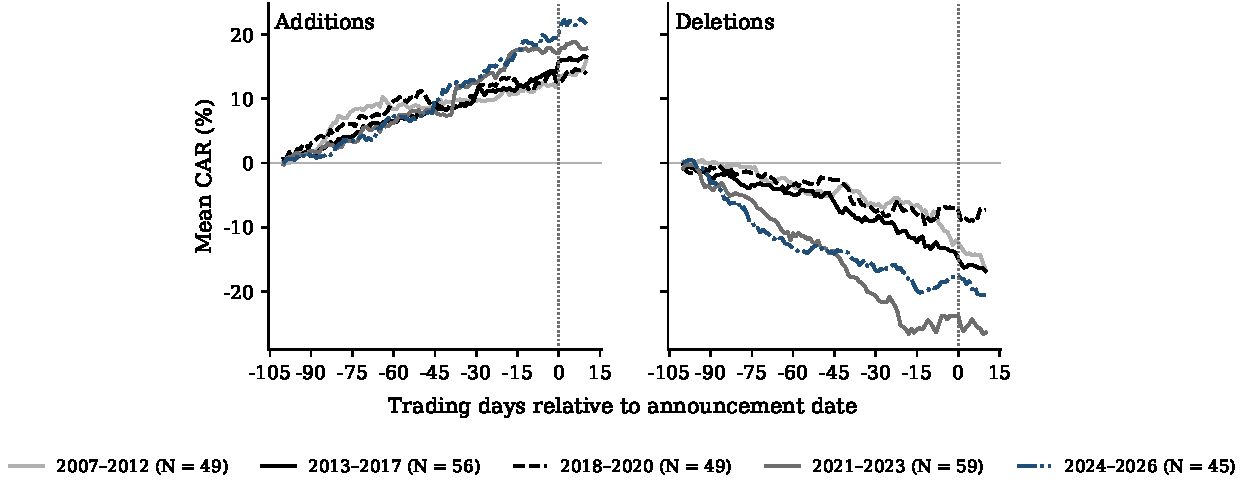
\includegraphics[width=0.85\textwidth]{fig_08_car_announcement.pdf}\end{center}
\end{frame}

\begin{frame}{Demand and price (anchor Figure 3)}
  \begin{center}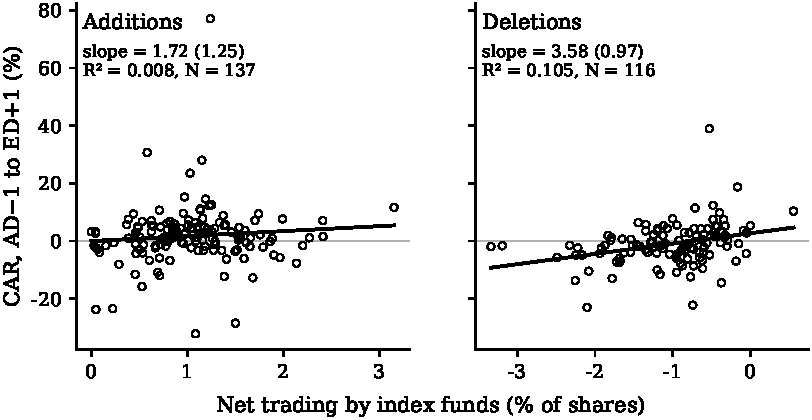
\includegraphics[width=0.78\textwidth]{fig_03_scatter.pdf}\end{center}
  \src{2019--2026. Deletions: $b = 3.6$ (1.0). Additions: $b = 1.7$ (1.3).}
\end{frame}

\begin{frame}{The five explanations on Swedish data}
  \footnotesize
  \begin{tabular}{p{2.6cm}p{10.4cm}}
    \toprule
    1 Composition & Controls explain nothing; the period pattern is unchanged \\
    2 Migrations & Not testable: no second Swedish index with its own trackers \\
    3 Predictability & Pre-announcement run-up rose from 12\% to 20\%; the 20-day window did not move \\
    4 General liquidity & Quoted spread fell from 0.27\% to 0.08\%; co-moves with the yearly effect \\
    5 Event liquidity & Volume on the day before the change rose from 10\% to 16\% of the window; non-index funds supply the stock \\
    \bottomrule
  \end{tabular}
\end{frame}

\end{document}
